% Version 1
% 23 July 2024
% 
% Данный шаблон подготовлен для сборника Прикладная математика и информатика, выпускаемого факультетом ВМК МГУ
% 
% This template is prepared for Prikladnaya Matematika i Informatika journal. The template is compatible with Computational Mathematics and Modeling journal template.
% 
% Prepared by Dmitry Sorokin (dsorokin@cs.msu.ru) 
%
%%%%%%%%%%%%%%%%%%%%%%%%%%%%%%%%%%%%%%%%%%%%%%%%%%%%%%%%%%%%%%%%%%%%%%
%%                                                                 %%
%% Please do not use \input{...} to include other tex files.       %%
%% Submit your LaTeX manuscript as one .tex document.              %%
%%                                                                 %%
%% All additional figures and files should be attached             %%
%% separately and not embedded in the \TeX\ document itself.       %%
%%                                                                 %%
%%%%%%%%%%%%%%%%%%%%%%%%%%%%%%%%%%%%%%%%%%%%%%%%%%%%%%%%%%%%%%%%%%%%%

%%=======================================================%%
%% to print line numbers in the margin use lineno option %%
%%=======================================================%%
%%======================================================%%
%% to compile with pdflatex/xelatex use pdflatex option %%
%%======================================================%%

\documentclass[pdflatex,sn-mathphys-gost]{pmi-jnl}
% \documentclass[pdflatex,sn-mathphys-num]{sn-jnl}

%%%% Standard Packages
%%<additional latex packages if required can be included here>

\usepackage[T2A]{fontenc}
\usepackage[russian]{babel}
\usepackage{anyfontsize}

\usepackage{graphicx}%
\usepackage{multirow}%
\usepackage{amsmath,amssymb,amsfonts}%
\usepackage{amsthm}%
\usepackage{mathrsfs}%
\usepackage[title]{appendix}%
\usepackage{xcolor}%
\usepackage{textcomp}%
\usepackage{manyfoot}%
\usepackage{booktabs}%
\usepackage{algorithm}%
\usepackage{algorithmicx}%
\usepackage{algpseudocode}%
\usepackage{listings}%
\usepackage{subcaption}%
\renewcommand\thesubfigure{\asbuk{subfigure}}
%%%%


%%======================================================%%
%% theorems
\newtheorem{theorem}{Теорема}%  meant for continuous numbers
%%\newtheorem{theorem}{Теорема}[section]% meant for sectionwise numbers
%% optional argument [theorem] produces theorem numbering sequence instead of independent numbers for Proposition
\newtheorem{proposition}[theorem]{Утверждение}% 
%%\newtheorem{proposition}{Утверждение}% to get separate numbers for theorem and proposition etc.
\newtheorem{example}{Пример}%
\newtheorem{remark}{Замечание}%
\newtheorem{definition}{Определение}%

\raggedbottom
%%\unnumbered% uncomment this for unnumbered level heads

\begin{document}

\author*[1]{\fnm{Савенкова} \sur{Н. П.}}\email{mknandrew@mail.ru}
\author*[1]{\fnm{Мокин} \sur{А. Ю.}}\email{mknandrew@mail.ru}
\author*[1]{\fnm{Удовиченко} \sur{Н. С.}}\email{nellya.udovichenko@gmail.com}
\author*[1]{\fnm{Сапожников} \sur{К. Э.}}\email{s02220529@gse.cs.msu.ru}
\author*[1]{\fnm{Ненахов} \sur{Н. Д.}}\email{nenakhov.neil@mail.ru}

\affil*[1]{\orgdiv{ВМК}, \orgname{Федеральное государственное бюджетное образовательное учреждение высшего образования «Московский государственный университет имени М.В.Ломоносова»}, \orgaddress{\street{Ленинские горы}, \city{Москва}, \postcode{119991}, \country{Российская Федерация}}}

\title[Математическое моделирование управляющих параметров электролизной ванны]{Математическое моделирование управляющих параметров электролизной ванны}

\abstract{В предлагаемой статье обсуждаются способы вычисления основных управляющих параметров работы электролизной ванны (криолитовое отношение, выход по току, потери выхода по току), значения которых отражают стабильность проведения процесса промышленного электролиза алюминия. Своевременное реагирование на изменение этих управляющих параметров способствует увеличению эффективности производства алюминия. Предлагается модифицированное уравнение Нернста-Планка, позволяющее вычислять концентрации основных ионов, возникающих в процессе электролиза, при помощи которых находится криолитовое отношение, а также модифицированы формулы нахождения параметра потери выхода по току. Приводится наглядная графическая иллюстрация проведенных численных экспериментов для МГД-стабильных и МГД-нестабильных режимов работы ванны.}

\keywords{Управляющие параметры, электролиз, математическое моделирование, численные методы.}

\received{01.01.2024}
\revised{02.02.2024}
\accepted{03.03.2024}

\maketitle

\section{Введение}\label{sec1}

Эффективное управление промышленным процессом электролиза алюминия требует внедрения автоматизированных систем управления – АСУТП, в которых в качестве начальных данных используются управляющие параметры, полученные в результате анализа физико-химических процессов, протекающих в электролизной ванне. Алюминиевая промышленность занимает в экономике России одно из ведущих мест. Высокие температуры и агрессивность среды, в которых происходит процесс электролиза алюминия, не позволяют провести измерения большинства параметров управления, необходимых для эффективной работы АСУТП. Наиболее перспективным направлением является разработка новых алгоритмов управления, построенных на понимании и моделировании технологического процесса электролитического получения алюминия. Это дает возможность автоматизировать отдельные контуры управления и оказывать поддержку технологу при принятии решений с целью увеличения выхода алюминия по току. 

Химический анализ состава электролита, позволяющий определить криолитовое отношение (КО), которое является одним из основных управляющих параметров, происходит 2 раза в неделю \cite{litlink:belo}. Для определения двух других важнейших управляющих параметров (выхода по току и потерь выхода по току) замер межполюсного расстояния, плотность анодного тока и поверхность раздела сред металл-электролит определяются весьма приблизительно. Это обстоятельство не позволяет с достаточной точностью определить параметры выхода по току и потери выхода по току и воспользоваться их значениями с целью внесения своевременных поправок в процесс управления электролизом алюминия.

Процесс электролиза алюминия сопровождается рядом физико-химических процессов, взаимовлияющих друг с другом, что наглядно отображено на рис. \ref{fig:vliyanie1}. Трёхмерная трёхфазная математическая модель процесса электролиза алюминия, на основе которой был реализован вычислительный комплекс, позволяющий достаточно точно вычислить величины, необходимые для определения управляющих параметров, учитывает взаимосвязь всех основных динамических процессов, происходящих в электролизной ванне. На рисунке \ref{fig:vliyanie2} изображена блок-схема этого вычислительного комплекса.

\begin{figure}[ht]
    \centering
    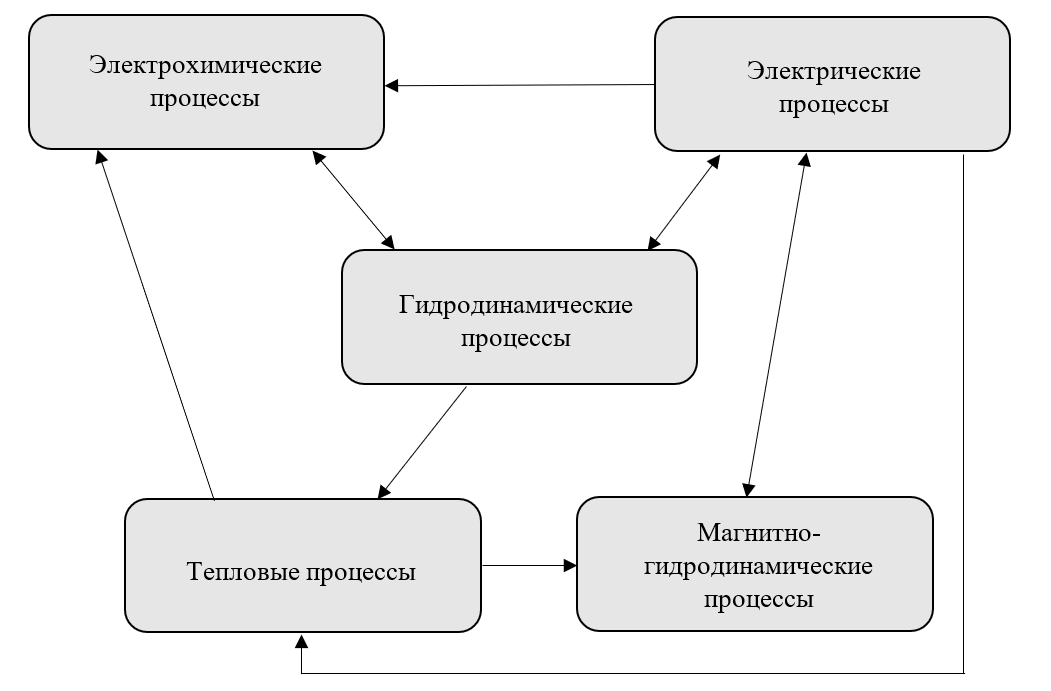
\includegraphics[width=1\textwidth]{схема взаимодействия.png}
    \caption{Взаимосвязь динамических процессов.}
    \label{fig:vliyanie1}
\end{figure}

\begin{figure}[ht]
    \centering
    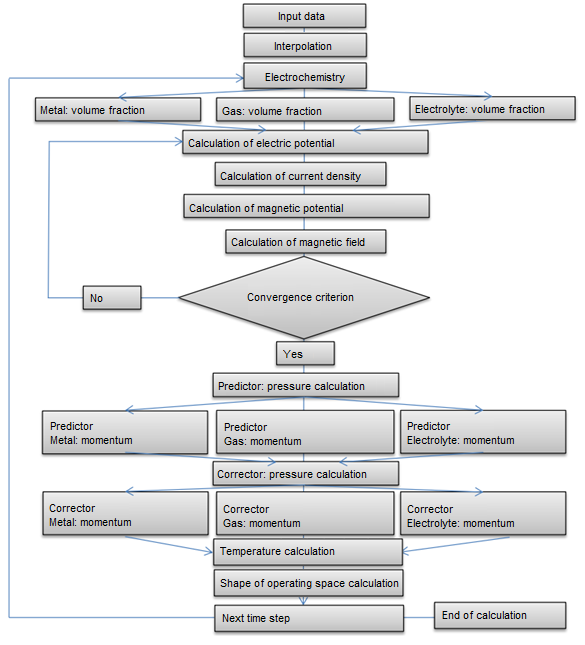
\includegraphics[width=1\textwidth]{блоксхема.png}
    \caption{ Блок-схема вычислительного комплекса.}
    \label{fig:vliyanie2}
\end{figure}

Для вычисления КО в любой интересующий момент времени требуется знать концентрации алюминия, натрия и фтора (блок «Электрохимия»), а также объёмные доли металла, электролита и газа, распределение плотности тока, потенциала и скорости в расплаве электролита, рассчитывающиеся каждый в своём блоке (см. рис. \ref{fig:vliyanie2}.). 

Для определения значений концентраций ионов используется уравнение Нернста-Планка, которое описывает изменения концентрации анионов и катионов химических элементов, возникающих в результате процесса электролиза \cite{litlink:burger}. Однако это уравнение не учитывает скорость движения среды. В работе \cite{litlink:damaskin} приводится модифицированное уравнение Нернста-Планка, учитывающее скорость движения заряженных частиц:

\begin{equation}\label{eq:NPeq}
	\frac{\partial C_i}{\partial t} = D_i\nabla^{2}C_i+D_i\frac{z_iF}{RT}div\big(C_i grad\phi\big) - \bar{v} \cdot gradC_i,
\end{equation}

В этом уравнении $\bar{v}$ – известная фиксированная скорость движения среды. Отметим, что при выводе уравнения (\ref{eq:NPeq}) предполагалось, что поле скоростей является соленоидальным, а температура --- постоянной. 

В настоящей работе учитывается взаимосвязь всех динамических процессов (см. рис. \ref{fig:vliyanie1}) и их зависимость от пространства и времени. В том числе зависимость температуры и коэффициента диффузии от пространственных координат и времени. Предлагается иная модификация уравнения Нернста-Планка. 

\section{Математическое моделирование криолитового отношения}

Ниже представлено модифицированное уравнение Нернста-Планка, которое используется для вычисления концентрации ионов, необходимых для расчёта КО

\begin{equation}\label{eq:NPeqmod}
	\frac{\partial C_i}{\partial t} = div\bigg(D_i gradC_i + D_i \frac{z_iF}{RT}C_igrad\phi\bigg) - div(C_i \bar{v}_{\text{эл}}),
\end{equation}

где $C_i$ – концентрация $i$-ого иона/катиона, $t$-время, $D_i (T)$ – коэффициент диффузии $i$-ого иона/катиона, $z_i$ – заряд $i$-ого иона/катиона, $F$ – постоянная Фарадея, $R$ – универсальная газовая постоянная, $T(t,x,y,z)$ – температура, $\phi (t,x,y,z)$ – потенциал электростатического поля, $\bar{v}_\text{эл}$ – скорость ионов.

Граничные условия на аноде и катоде

\begin{equation}\label{eq:granuslac}
	\big(\nabla C_i + K_i C_i \nabla \phi \big) \cdot \bar{n} = G_i, 
\end{equation}

где $K_i$ – коэффициент, определяющийся типом ионов,  $G_i$ зависит от плотности анодного (катодного) тока, $\bar{n}$ – нормаль к границе.

Граничные условия на стенках ванны

\begin{equation}\label{eq:granuslstenki}
	\big(\nabla C_i + K_i C_i \nabla \phi \big) \cdot \bar{n} = 0,
\end{equation}

Концентрация ионов натрия находится из условия электронейтральности среды

\[ \sum\limits_{i=1}^6 z_iC_i = 0. \]

Концентрацию ионов алюминия предлагается находить из уравнения 

\[ \frac{\partial C_{Al}}{\partial t} = \frac{j_a}{F} - div(C_{Al} \bar{v}_{\text{эл}}), \]
\\
где $j_a$ - плотность тока на аноде.

Начальные условия для каждого иона известны, начальные условия для алюминия определяются в зависимости от его фазовой доли. 

Таким образом, математическая постановка задачи вычисления КО заключается в решении уравнения (\ref{eq:NPeqmod}) с граничными условиями (\ref{eq:granuslac}), (\ref{eq:granuslstenki}). Потенциал $\phi(t,x,y,z)$ и скорость $v(t,x,y,z)$ находятся при помощи основного вычислительного комплекса в каждый момент времени.

Задача (\ref{eq:NPeqmod})-(\ref{eq:granuslstenki}) решается разностным методом, при этом уравнение (\ref{eq:NPeqmod}) аппроксимируется со вторым порядком точности по пространству и по времени.

Анализ проведённой серии численных экспериментов позволил изучить пространственное распределение КО. 
Ниже представлены результаты расчёта трёхмерной задачи в плоскостном срезе рабочего плоскости XY на глубине 3 см от подошвы анода. На рисунке \ref{fig:veloxy} представлен график векторного поля скоростей в расплаве криолита на высоте 39 см от дна ванны (на расстоянии 3 см от подошвы анода). Можно заметить, что завихрения образуются по всей площади ванны: обводящий по периметру вихрь, а также интенсивные вихри в центре сечения.

На рисунке \ref{fig:crxy} представлено распределение значений КО. Все вычисленные значения КО соответствуют известному диапазону стабильной работы ванны (2.6-2.8) и подтверждается экспериментальными наблюдениями. 

\begin{figure}[ht]
    \centering
    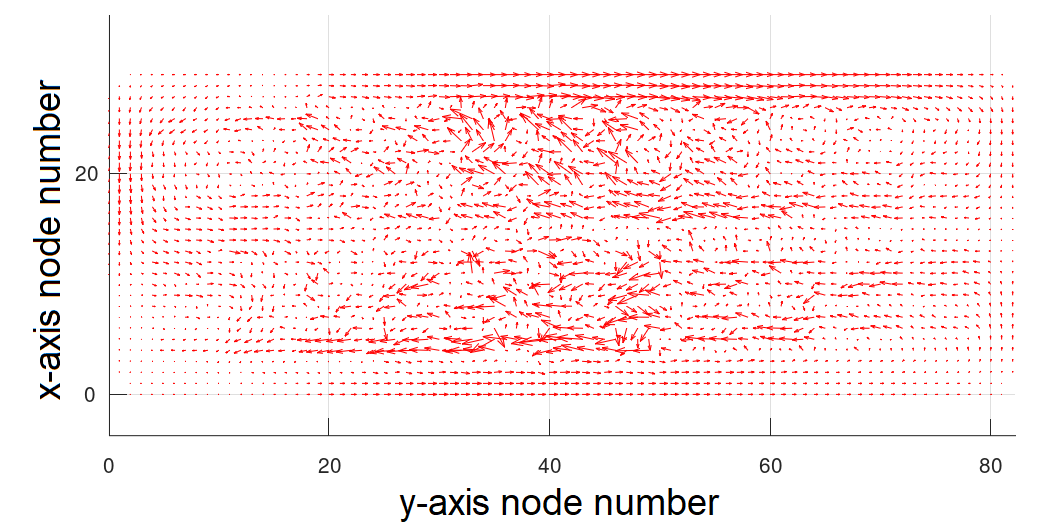
\includegraphics[width=100mm]{veloxy_art.png}
    \caption{Векторное поле скоростей в плоскости XY.}
    \label{fig:veloxy} 
\end{figure}

\begin{figure}[ht]
    \centering
    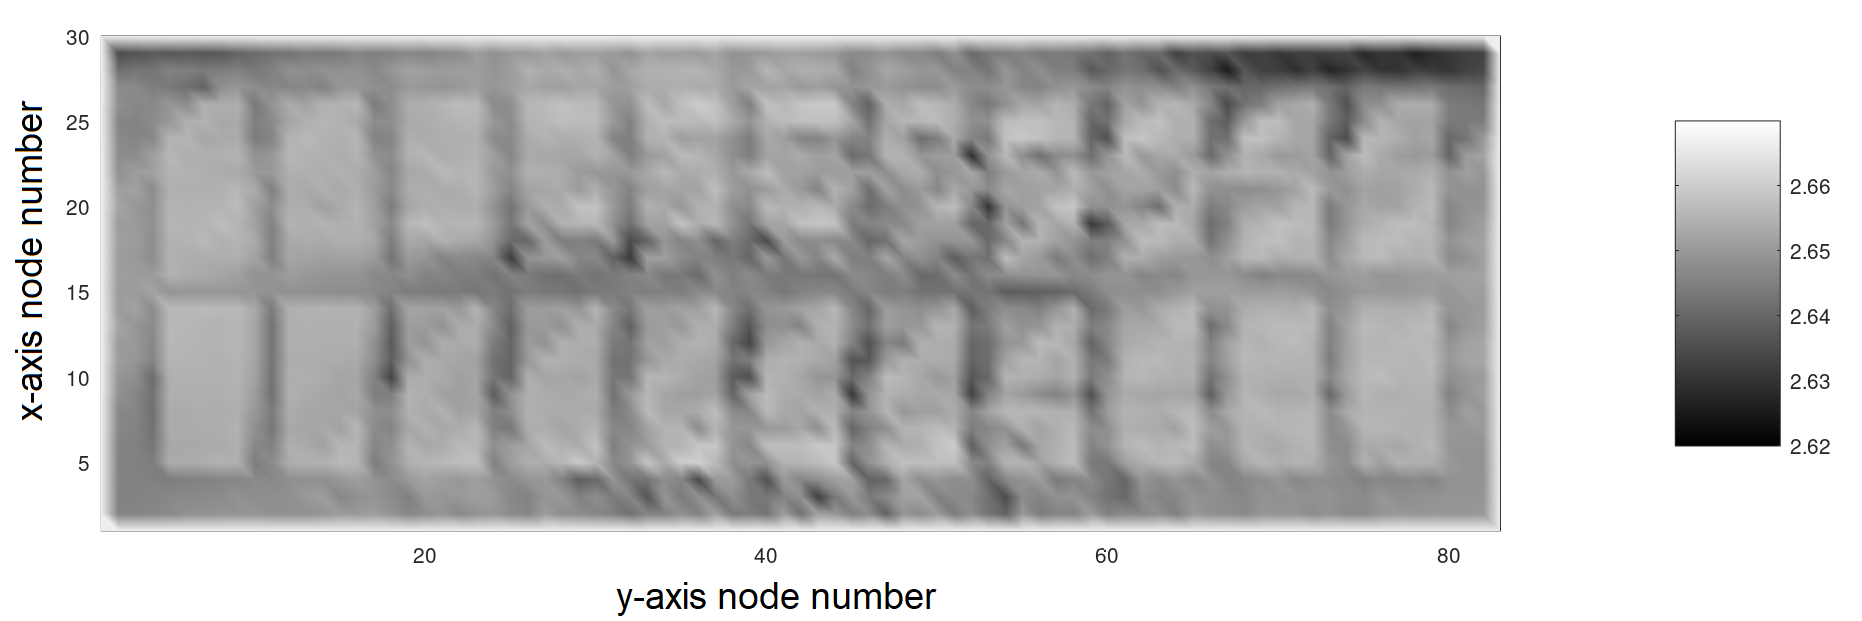
\includegraphics[width=100mm]{crxy_art.png}
    \caption{Распределение значений криолитового отношения в плоскости XY.}
    \label{fig:crxy} 
\end{figure}

На рисунке \ref{fig:veloxz} представлен график векторного поля скоростей в расплаве криолита. Наблюдается обводящий по периметру поток и небольшие вихревые образования у левого борта ванны.

Результаты численного эксперимента для сечения рабочего пространства плоскостью XZ на расстоянии 1,34 м от короткого борта промышленной ванны представлены на рисунке \ref{fig:crxz}. Наглядно видно, что соответствующее распределение КО для скоростей, представленных на рис. 5, фактически однородно по всей плоскости сечения и принадлежит диапазону устойчивости работы ванны. 

\begin{figure}[ht]
    \centering
    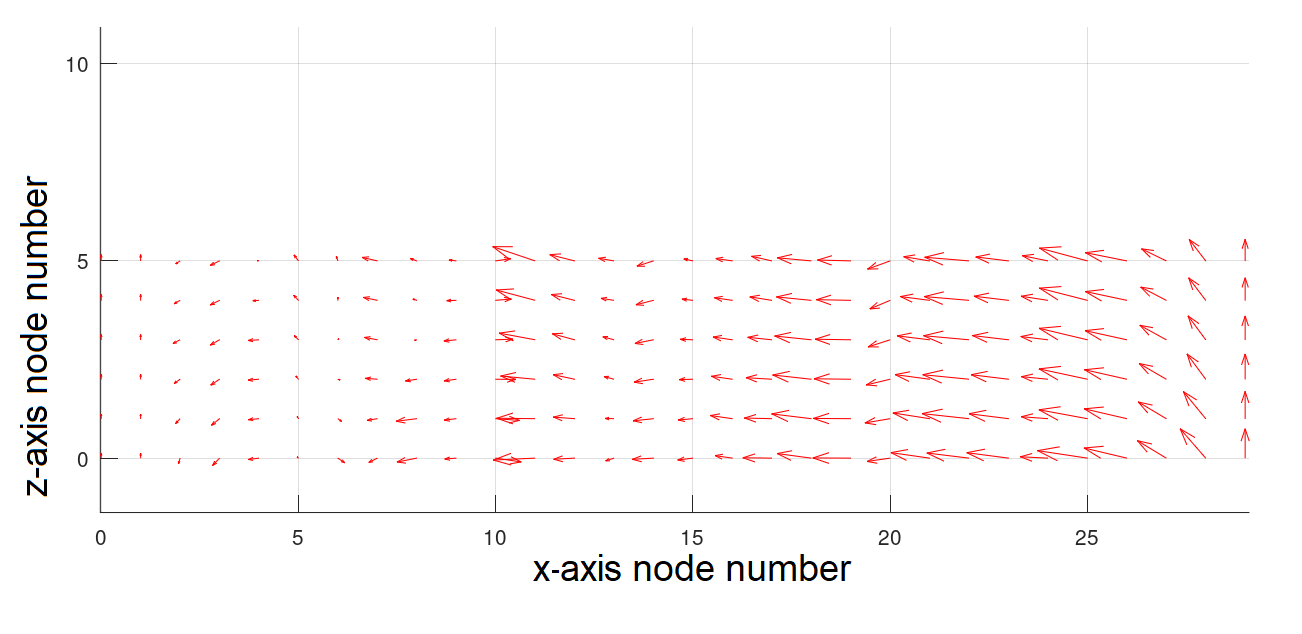
\includegraphics[width=110mm]{veloxz_art.png}
    \caption{Векторное поле скоростей в плоскости XZ.}
    \label{fig:veloxz} 
\end{figure}

\begin{figure}[ht]
    \centering
    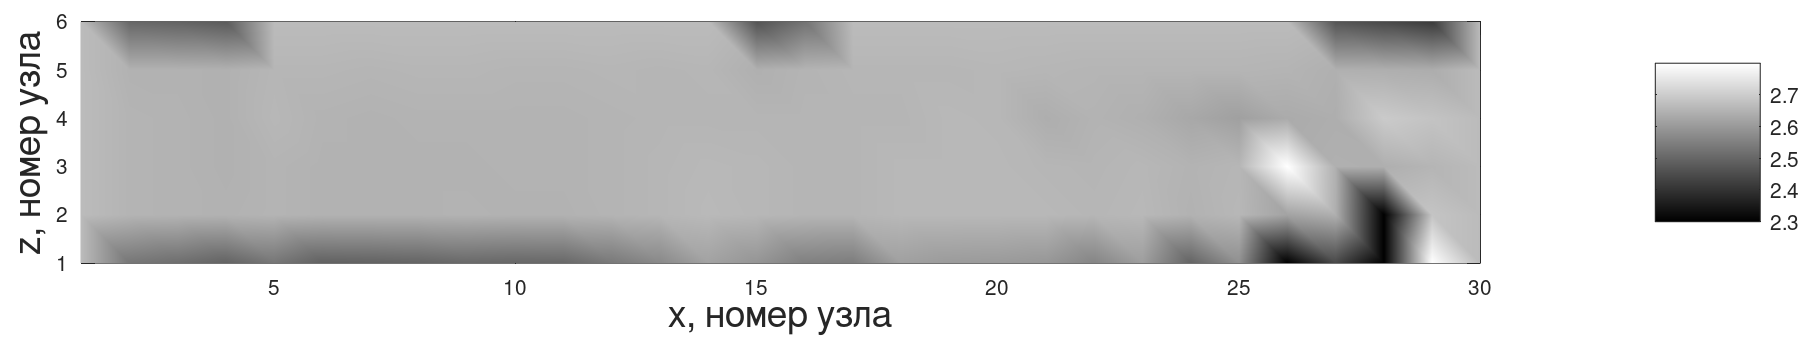
\includegraphics[width=90mm]{heatmapxz_art.png}
    \caption{Распределение значений криолитового отношения в плоскости XZ.}
    \label{fig:crxz} 
\end{figure}

На рисунках \ref{fig:veloyz}, \ref{fig:cryz} демонстрируются результаты численного эксперимента для сечения рабочего пространства плоскостью YZ, находящегося между длинным бортом и анодом на расстоянии 22 см от длинного борта промышленной ванны.	

На рисунке \ref{fig:veloyz} представлен график векторного поля скоростей в расплаве криолита. Видно, что в этой плоскости значения скоростей невелики, вихрей не наблюдается. На рисунке \ref{fig:cryz} представлено соответствующее распределение значений КО.

Как и следовало ожидать, значения КО в плоскости сечения примерно одинаковы (КО = 2,65) и входят в диапазон значений устойчивой работы ванны. 

Таким образом, вихревые образования в поле распределения скоростей приводят к неоднородному распределению КО в рабочем пространстве. На практике это означает, что результат химического анализа взятой пробы сильно зависит от места взятия пробы в случае наличия вихревого движения скоростей и не зависит от места взятия пробы при безвихревом движении среды.

\begin{figure}[ht]
    \centering
    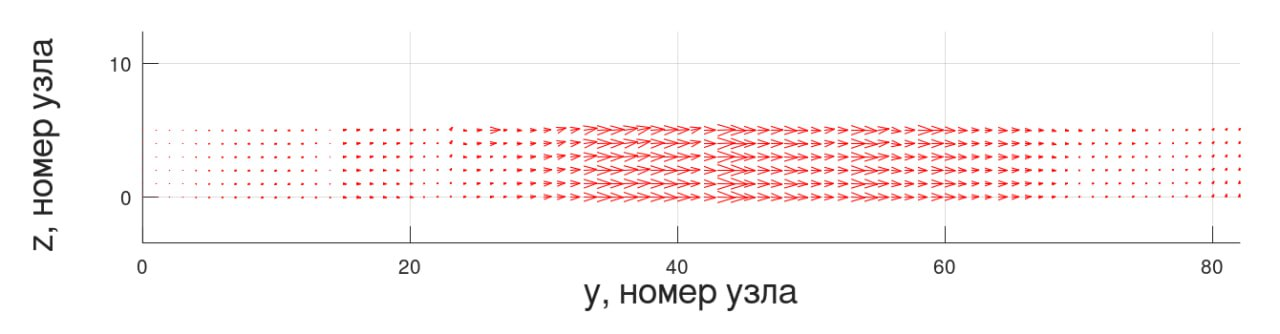
\includegraphics[width=110mm]{veloyz_art.png}
    \caption{Векторное поле скоростей в плоскости XZ.}
    \label{fig:veloyz} 
\end{figure}

\begin{figure}[ht]
    \centering
    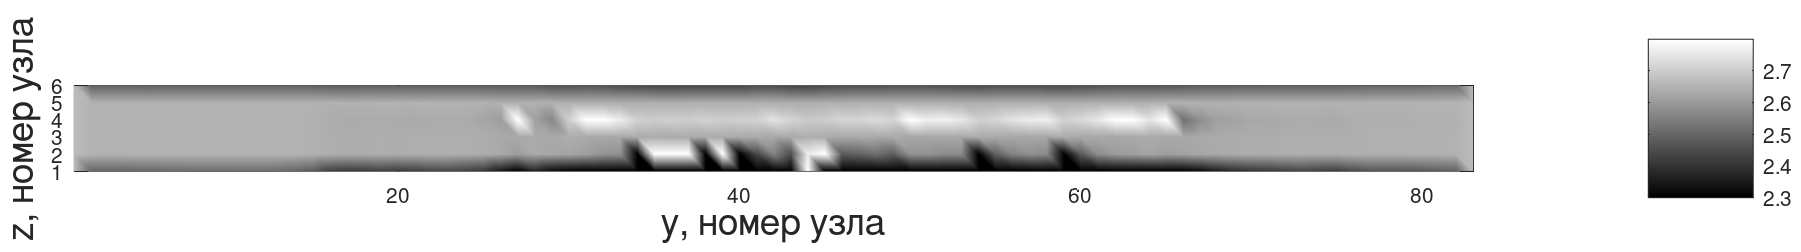
\includegraphics[width=90mm]{heatmapyz_art.png}
    \caption{Распределение значений криолитового отношения в плоскости XZ.}
    \label{fig:cryz} 
\end{figure}

\section{Вычисление управляющих параметров выхода по току и потери выхода по току}

Управляющие параметры выхода по току $\eta$ и потери выхода по току $\Delta \eta$ наглядно отражают эффективность выхода по току алюминия при различных режимах работы электролизной ванны.

Теоретическое количество алюминия, которое должно получиться при электролизе, вычисляется по закону Фарадея

\begin{equation}\label{eq:farad}
	M = F \cdot I \cdot t,
\end{equation}

где $F$ - постоянная Фарадея, $I$ - сила тока, $t$ - время.

Однако количество произведённого металла всегда несколько меньше теоретического значения.

Экспериментальные исследования показывают, что выход по току $\eta$ зависит от большого числа параметров: температуры, межполюсного расстояния (МПР) - расстояния между подошвой анода и границей раздела сред металл-электролит, плотности тока, геометрии рабочего пространства электролизёра, электромагнитных сил \cite{litlink:belo}.

На практике в АСУТП применяется следующая эмпирическая формула \cite{litlink:VAMI}

\begin{equation}\label{eq:f1}
	\eta = \bigg(1-2567 \cdot \frac{S^{0,21}_{anod}}{i^{0,58}_{a}\cdot L \cdot e^{\frac{12940}{T_e}}}\bigg) \cdot 100,
\end{equation}

где $S$ площадь ванны, $i$ плотность тока, $L$ - минимальное межполюсное расстояние, $T_e$ - температура электролита.

При этом значения анодной плотности тока, температуры электролита и МПР определяются экспериментально в нескольких отдельных точках рабочего пространства ванны.
Таким образом точность вычисления выхода по току по формуле (\ref{eq:f1}) напрямую зависит от точности входящих в неё параметров. Поскольку на практике значениям этих параметров соответствует большая погрешность, то величина $\eta$ по формуле (\ref{eq:f1}) вычисляется с большой погрешностью. Трёхмерное трёхфазное математическое моделирование \cite{litlink:kalmykov} позволяет исследовать распределение в рабочем пространстве ванны всех параметров, входящих в формулу (\ref{eq:f1}), с достаточно большой точностью и изучить распределение $\eta$ и $\Delta\eta$, на основе которого можно сделать достоверную оценку эффективности производства алюминия в различные моменты времени.

В зависимости от режима работы электролизной ванны процесс электролиза может быть МГД-стабилен или МГД-нестабилен. В случае МГД-нестабильной работы ванны расстояние между анодом и катодом может быть критически мало, что ведёт к резкому уменьшению выхода по току. МГД-нестабильность всегда соответствует анодному эффекту (большое скопление углекислого газа под анодами, увеличивающего сопротивление среды), который происходит несколько раз в сутки. МГД-нестабильность развивается при одновременной замене 11 и 22 анодов. В таблице \ref{table:vihPoToku} приводятся результаты вычисления величины выхода по току в моменты времени $t_1$ и $t_2$ $(t_2>t_1)$ при МГД-стабильности и МГД-нестабильности ванны. 

%тут должна быть таблица 1 (выход по току) (на самом деле 2 потому что свою я не сделал ещё)
\begin{table}[h]
\caption{Выход по току $\eta$ для минимального значения МПР ($t_1 < t_2$).} \label{table:vihPoToku}
\centering
\begin{tabular}{|c|c|}
\hline
Режим работы ванны &Выход по току	\\
\hline
МГД стабильный режим работы &	\\
Момент времени $t_1$			&90.646	\\ 
Момент времени $t_2$		&93.594	\\  
\hline
Выемка 11 и 22 анодов &	\\
Момент времени $t_1$		&89.638	\\  
Момент времени $t_2$		&91.365	\\  
\hline
Анодный эффект &	\\
Момент времени $t_1$	&87.048	\\  
Момент времени $t_2$	&90.037	\\  
\hline
\end{tabular}
\end{table}

\begin{figure}[ht]
    \centering
    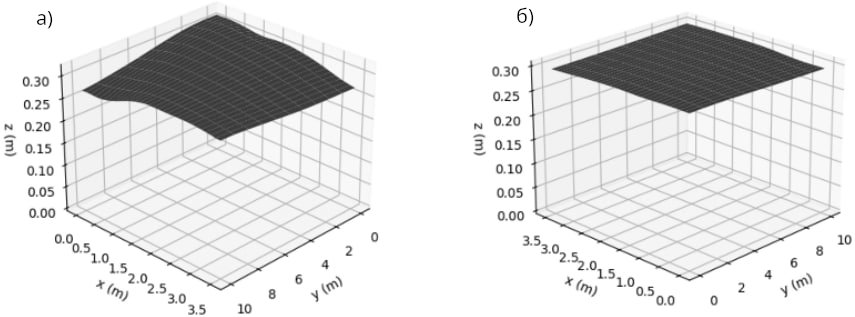
\includegraphics[width=150mm]{спокойная поверхность.png}
    \caption{Поверхность раздела сред металл-электролит при МГД-стабильной работе ванны в моменты времени $t_1$(а) и $t_2$(б).}
    \label{fig:stab} 
\end{figure}

На рисунке 10 представлены поверхности раздела сред металл-электролит при выемке анодов в момент времени $t_1$ и $t_2$ для которых вычислялось значения выхода по току в таблице 1.

\begin{figure}[ht]
    \centering
    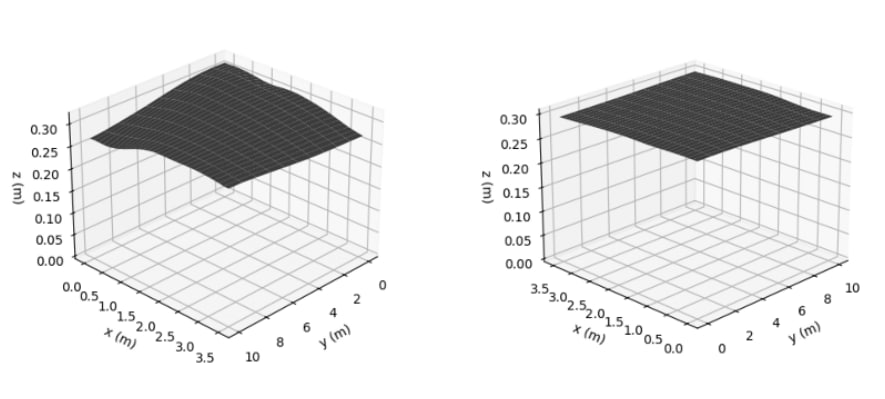
\includegraphics[width=150mm]{Выемка анодов поверхность.png}
    \caption{Поверхность раздела сред металл-электролит при при выемке анодов.}
    \label{fig:viemkaanod} 
\end{figure}

На рисунке 11 представлены поверхности раздела сред металл-электролит при анодном эффекте в момент времени $t_1$ и $t_2$ для которых вычислялось значения выхода по току в таблице 1.

\begin{figure}[ht]
    \centering
    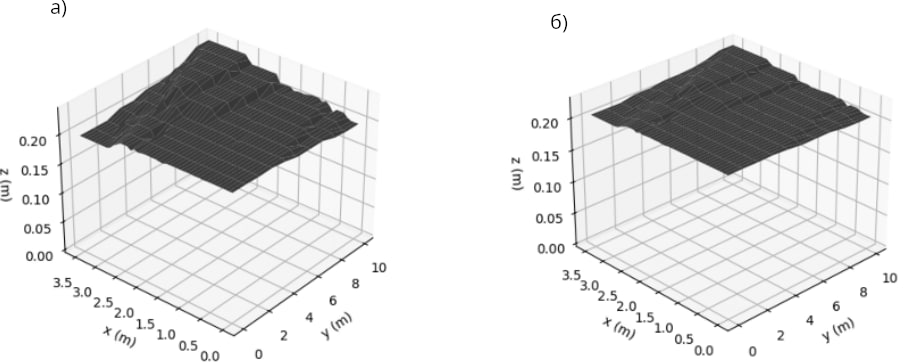
\includegraphics[width=150mm]{Анодный эффект поверхность.png}
    \caption{Поверхность раздела сред металл-электролит при анодном эффекте.}
    \label{fig:anodeffect}
\end{figure}

Несмотря на то, что абсолютные значения изменения выхода по току и изменения потерь по току отличаются, они имеют общую тенденцию на уменьшение выхода по току при искривлении поверхности. Такой результат можно было ожидать, поскольку формулы зависят от совершенно разных параметров, сильно связанных между собой в электролизёре в каждый момент времени, но по сути являющимися независимыми в расчётах по формуле (\ref{eq:f1}). Например, при возникновении анодного эффекта резко возрастает за доли секунды напряжение, повышается температура в электролизёре, уменьшается плотность тока. При замене пары 11 и 22 анодов в электролизёре происходит перераспределение силы тока в ванне и рост амплитуды колебания границы раздела сред металл-электролит в области выемки анодов. В этих двух случаях за малое время невозможно провести замеры входящих в формулу (\ref{eq:f1}) параметров. Тем не менее результаты, представленные в таблице \ref{fig:stab}, отражают общие тенденции по увеличению выхода по току при более стабильном режиме работы ванны.

В работе \cite{litlink:derkach2} представлена полуэмпирическая формула выхода по току

\begin{equation} \label{eq:f2}
	\Delta \eta = (1- \eta_0) \cdot \frac{l}{S} \cdot \int\limits_Z \frac{ds}{H(x,y)}
\end{equation}

Однако практическая реализация формулы (\ref{eq:f2}) зависит от точности определения поверхности раздела сред металл-электролит Z, а также требует достаточно точного вычисления поверхностного интеграла. 

При этом величина МПР, как и в формуле (\ref{eq:f1}), определяется очень грубо (по характеру оплава опущенного в электролизную ванну стержня). Поэтому практическое использование формулы (\ref{eq:f2}) весьма затруднительно. Более того, как показали проведённые в работе исследования, формула (\ref{eq:f2}) является противоречивой, поскольку в случае выемки анодов (см. рис. \ref{fig:viemkaanod}) в момент времени $t_2$, т.е. при спокойной поверхности раздела сред металл-электролит, значение  потерь выхода по току $\Delta\eta_2 = 0.0099$, а в момент времени $t_1$ при сильном возмущении границы раздела сред значение потери выхода по току $\Delta\eta_1 = 0.0074$, что противоречит здравому смыслу.  Таким образом, применение формулы (\ref{eq:f2}) не является целесообразным.

Авторами предлагается модифицированная формула потерь выхода по току 

\begin{equation} \label{eq:modf2}
	\Delta \eta = (1- \eta_0) \cdot \frac{1}{S} \cdot \int\limits_Z \frac{l(x,y) ds}{H(x,y)},
\end{equation}
в которой значения величин $l(x,y)$,$ H(x,y)$ в каждый момент времени определяются при помощи трёхмерного математического моделирования.

Вычисление поверхностного интеграла предлагается проводить при помощи метода триангуляции по формулам 

\begin{equation}\label{eq:triangsquare}
	{S_{\triangle_{i,j}^{1,2}}} = \frac{1}{2} \cdot |\bar{a} \times \bar{b}|
\end{equation}

\begin{align}
	F^1_{i,j} = \frac{1}{3}(f_{i,j}+f_{i,j+1}+f_{i+1,j}), \label{eq:triangf1}\\
	F^2_{i,j} = \frac{1}{3}(f_{i+1,j+1}+f_{i,j+1}+f_{i+1,j}). \label{eq:triangf2}
\end{align}

\begin{align}\label{eq:trint}
	I \approx \sum_{i=0}^{N-1} \sum_{j=0}^{M-1} I_{i,j} = \sum_{i=0}^{N-1} \sum_{j=0}^{M-1} (S_{\triangle_{i,j}^1} \cdot F_{i,j}^1 + S_{\triangle_{i,j}^2} \cdot F_{i,j}^2)
\end{align}

Поверхность разбивается на элементарные треугольники $\triangle_{i,j}^{1,2}$, как показано на рисунке \ref{fig:triangles}, площадь каждого из этих элементарных треугольников вычисляется по формуле (\ref{eq:triangsquare}), где $\bar{a}$ и $\bar{b}$ — векторы, совпадающие со сторонами треугольника $\triangle_{i,j}^{1,2}$. Для каждого элементарного треугольника вычисляются значения подынтегральной функции по формулам (\ref{eq:triangf1}) и (\ref{eq:triangf2}) соответственно. Тогда значение поверхностного интеграла вычисляется по формуле (\ref{eq:trint}).

\begin{figure}[ht]
    \centering
    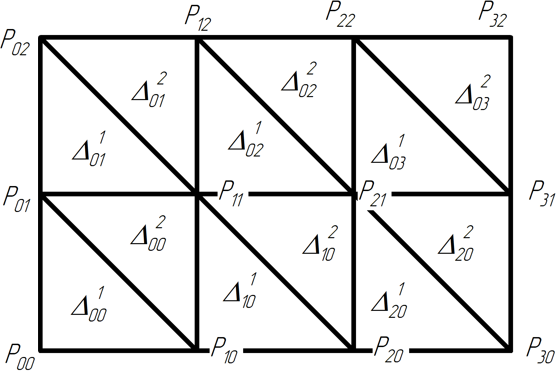
\includegraphics[width=150mm]{triangul.png}
    \caption{Триангуляция расчетной области.}
    \label{fig:triangles} 
\end{figure}

Точность вычисления поверхностного интеграла по формулам (\ref{eq:triangsquare}) – (\ref{eq:trint}) имеет второй порядок и исследовалась численно на сгущающихся сетках.

Численный расчёт значений потерь выхода по току в случаях МГД-стабильной работы ванны $(\Delta\eta_1)$, при выемке анодов $(\Delta\eta_2)$ и анодном эффекте $(\Delta\eta_3)$ в момент времени $t_1$ показал, что 

\begin{equation}
	\Delta\eta_1 = 0.00674 < \Delta\eta_2 = 0.00945 < \Delta\eta_3 = 0.01188, \notag
\end{equation}

откуда следует, что наибольшие потери выхода по току соответствуют анодному эффекту, а наименьшие – МГД-стабильному режиму работы ванны. Этот вывод соответствует практическим наблюдениям.

Аналогичные вычисления были проведены в момент времени $t_2$, которые показали, что

\begin{equation}
	\Delta\eta_1 = 0.00667 < \Delta\eta_2 = 0.00928 < \Delta\eta_3 = 0.01173. \notag
\end{equation}

Процентные изменения потерь выхода по току в моменты времени $t_1$ и $t_2$ представлены в таблице \ref{table:ismineniep}. 

\begin{table}[h]
\centering
\caption{Процентное изменение выхода потерь алюминия по току.}
\begin{tabular}{|c|c|}
\hline
Режим работы ванны & Процентное изменение \\
 					& потерь по току \\
\hline
МГД стабильный режим работы (рис \ref{fig:stab}) & 1.038	\\
\hline
Выемка 11 и 22 анодов (рис \ref{fig:viemkaanod}) &	1.799\\
\hline
Анодный эффект (рис \ref{fig:anodeffect}) & 1.262	\\
\hline
\end{tabular}
\label{table:ismineniep}
\end{table}

Таким образом, из приведенных расчетов следует, что в оба момента времени прослеживается закономерность увеличения потерь по току при МГД-нестабильности. Причем потери при выемке анодов меньше, чем при анодном эффекте. В то же время при стабилизации поверхности раздела сред, которая происходит в промежутке времени ($t_1, t_2$), потери уменьшаются для любого режима работы ванны.

Ниже представлены результаты численных расчётов, иллюстрирующих распределение величины потери выхода по току в момент времени $t_1$ и разных режимах работы ванны. Для каждого элементарного треугольника $\Delta^{1,2}_{i,j}$ проводится расчёт величины потери выхода по току $(\Delta\eta)_{i,j}$ для соответствующей формы поверхности раздела сред металл-электролит (см. рис. \ref{fig:stab} - \ref{fig:anodeffect}). На рис. \ref{fig:stabrasp} - \ref{fig:anodeffectrasp} представлены соответствующие распределения потерь выхода по току для границ раздела сред металл-электролит в случае МГД-стабильной и МГД-нестабильной работы ванны.

\begin{figure}[ht]
    \centering
    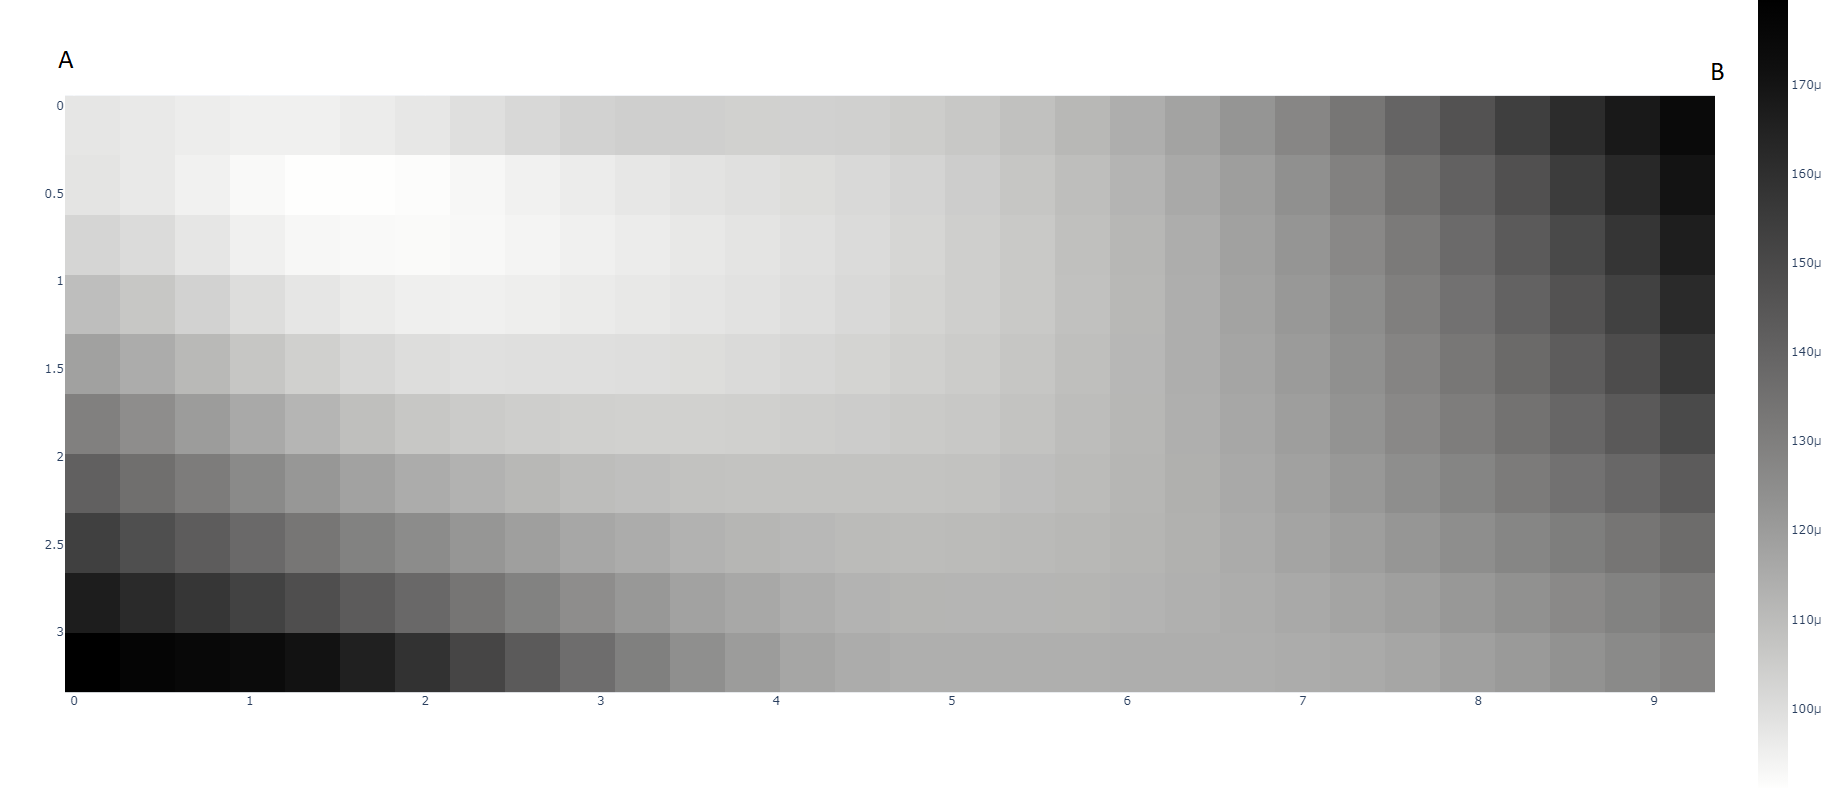
\includegraphics[width=150mm]{h.png}
    \caption{Распределение потерь по току для МГД-стабильного режима работы.}
    \label{fig:stabrasp}
\end{figure}

\begin{figure}[ht]
    \centering
    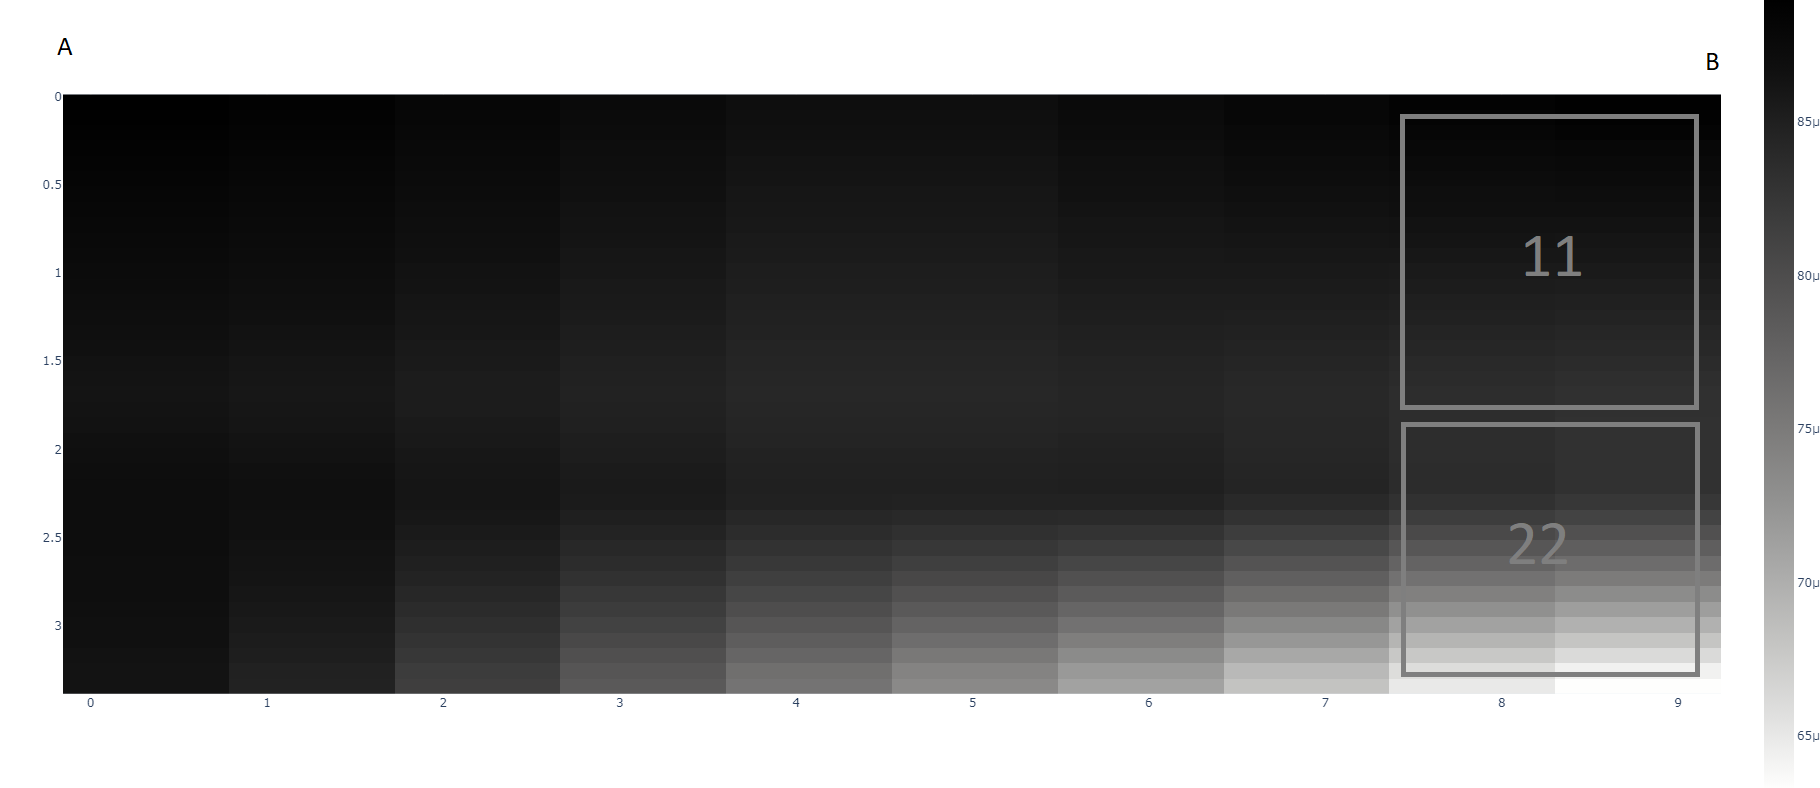
\includegraphics[width=150mm]{выемка анодов.png}
    \caption{Распределение потерь по току для выемки 11 и 22 анодов.}
    \label{fig:viemkaanodrasp} 
\end{figure}

\begin{figure}[ht]
    \centering
    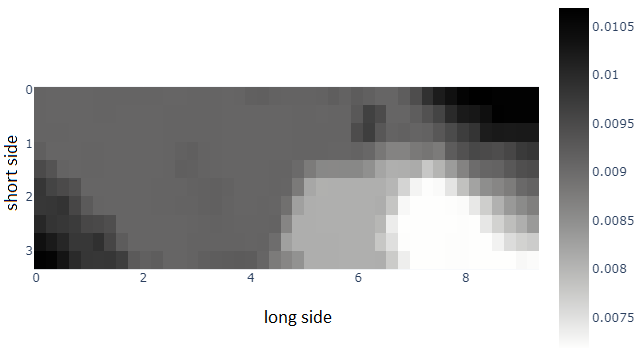
\includegraphics[width=150mm]{анодный эффект.png}
    \caption{Распределение потерь по току для анодного эффекта.}
    \label{fig:anodeffectrasp} 
\end{figure}

Анализ проведённых численных экспериментов позволяет сделать выводы о корреляции результатов расчетов и результатов лабораторных исследований стабильности режима работы ванны.

\section{Заключение}

Эффективность работы электролизной ванны диктует необходимость развития инструментов управления технологическим процессом с целью быстрого реагирования на изменения режима работы ванны. Значения основных управляющих параметров (криолитовое отношение, выход по току, потери по току) наглядно отражают физико-химические процессы, происходящие в среде электролита, и позволяют судить о применении тех или иных технологических решений с целью стабилизации режимов работы ванны. Предложенные в работе методы вычисления управляющих параметров ванны позволяют вычислять и своевременно реагировать на их изменения, что в свою очередь способно значительно увеличить эффективность и прибыльность производства.

\section*{Авторские декларации}

\subsection*{Финансирование}

Отсутствует.

\subsection*{Доступность данных и программного кода}

Недоступны.

\subsection*{Конфликт интересов}

Отсутствует.

\subsection*{Вклад авторов}

Н. П. Савенкова -- разработка математических методов, написание текста статьи.

А. Ю. Мокин -- численные эксперименты, написание текста статьи.

Н. С. Удовиченко -- численные эксперименты.

К. Э. Сапожников-- численные эксперименты, написание текста статьи.

Н. Д. Ненахов -- численные эксперименты, написание текста статьи.

% Вставить недостающую ссылку #TODO
\bibliography{pmi-bibliography}% common bib file

\end{document}
